\chapter{Planificación y costes} \label{planificacion_chap}
En este capítulo se comentará los requisitos que se diseñaron inicialmente y la descomposición del proyecto en \textit{Sprints}. Se hablará sobre los costes del proyecto (humanos y materiales) y se analizarán los resultados de cada \textit{Sprint} por separado. 
\section{Recursos}
En esta sección se enumerarán los recursos de los que se dispuso para la realización del proyecto. Habrá tres apartados: humanos, materiales y \textit{Software}.
\subsection*{Recursos humanos}
Los recursos humanos en este proyecto han sido muy pocos, como hemos venido comentando hasta ahora. Constarían de:
\begin{itemize}
\item \textbf{El jefe de proyecto:} En este caso es el profesor, tutor de este trabajo de fin de grado. Realizó las tareas de supervisión, \textit{Scrum Master} y analista.
\item \textbf{El equipo de desarrollo:} en este caso está conformado simplemente por el alumno. El cual tuvo que realizar todas las tareas de análisis, diseño, implementación, pruebas y documentación.
\end{itemize}
\subsection*{Recursos materiales}
En cuanto a los recursos materiales empleados, se dispuso de las siguientes herramientas:
\begin{itemize}
\item Ordenador con sistema operativo \textit{macOS}, imprescindible para programar aplicaciones para dispositivos móviles con sistema operativo \textit{iOS}. El modelo concreto fue un \textit{MacBook Pro} de 2017 con sistema operativo \textit{macOS High Sierra}. Al ser portátil, facilitó el transporte a las reuniones con el director de proyecto, así como permitió trabajar en cualquier lugar.
\item \textit{Smartphone} de la marca \textit{Apple} con sistema operativo \textit{iOS} 12 beta, sirvió para realizar pruebas de la aplicación sobre un dispositivo real. El modelo concreto es un \textit{iPhone SE}.
\item \textit{Beacons} utilizados para calibrar el entorno, aunque podrían haberse prescindido de ellos ya que se puede calibrar solamente con \textit{WiFi}. El modelo concreto es \textit{iBSK105} de la marca \textit{Accent Systems}.
\end{itemize}
\subsection*{Recursos software}
\begin{itemize}
\item \textit{IDE} para programar aplicaciones \textit{iOS}, el programa se llama \textit{Xcode} y sólo puede ejecutarse en máquinas con \textit{macOS}.
\item Simuladores para ejecutar y probar la aplicación más rápidamente sin necesidad de utilizar un dispositivo físico, el \textit{IDE} comentado anteriormente ya incluye simuladores de gran cantidad de \textit{iPhones} y \textit{iPads} con diversas versiones de \textit{iOS}.
\item Programas para la generación de iconos en formato \textit{PDF}, se ha elegido la aplicación \textit{IconJar} en su versión gratuita de prueba y fue suficiente para descargar una cantidad importante de iconos en varios colores.
\item Programas de diseño de interfaces de aplicaciones móviles, en este proyecto se utilizó \textit{Adobe Xd} en su versión gratuita.
\item El programa \textit{Postman} que fue utilizado para probar todas las peticiones antes de su incorporación definitiva al proyecto, en su versión gratuita.
\item Plataforma \textit{online} ofrecida por \textit{Firebase}, en este caso en particular hemos utilizado las funcionalidades de base de datos, de autenticación y de ejecución de código \textit{Backend}, pero tiene muchas más.
\item Plataforma \textit{Situm} para la gestión de mapas interiores, para calibrar sus entornos y obtener la posición en los mismos. Tiene varias herramientas, pero en este caso se han utilizado el \textit{Dashboard} para subir los planos y la aplicación móvil para \textit{Android} \textit{SitumMapsTool} para calibrar los entornos.
\end{itemize}

\section{Planificación inicial}
En esta sección se muestra la descomposición en \textit{sprints} del proyecto y sobre como se llevó a cabo un desarrollo incremental, obteniendo resultados funcionales al final de cada iteración.
En la figura~\ref{fig:gantt_inicial} se puede ver la representación temporal de los \textit{sprints} y sus correspondientes hitos, a lo largo del tiempo.
\begin{figure}[tbp]
\begin{center}
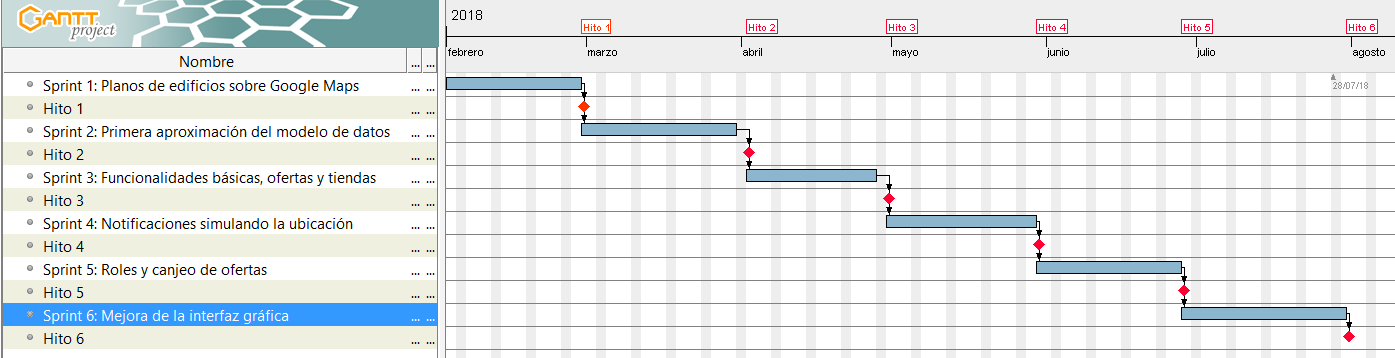
\includegraphics[scale=0.5]{figures/ganrr.png}
\caption{Diagrama de \textit{Gantt} de la planificación inicial.
\label{fig:gantt_inicial}}
\end{center}
\end{figure}

\subsection{\textit{Sprint} 1: Prototipo \textit{iOS} con localización en interiores}
En este \textit{sprint}, se suben a \textit{Situm} los planos interiores de varios edificios y se crea una aplicación móvil sencilla que obtiene estos planos y los superpone sobre un mapa de \textit{Google Maps}. Básicamente se sustituye el sistema de mapas interiores de \textit{Google} por uno propio, creando unos botones que permiten cambiar de piso y una caché que almacena las imágenes descargadas de \textit{Situm}. El \textit{sprint} se descompone en las siguientes tareas:
\begin{itemize}
\item Obtención de las \textit{API Keys} de \textit{Situm} y de \textit{Google Maps} para poder añadir estos servicios a nuestra aplicación.
\item Se sigue la guía para incorporar el \textit{SDK} de la plataforma \textit{Situm} a la aplicación \textit{iOS}. En este manual se indica como descargar todos los edificios y la información relativa a ellos: nombre, plantas, planos, etcétera.
\item Una vez obtenidos los edificios, sus planos se superponen sobre el mapa, sustituyendo los planos de interiores de \textit{Google} por los de \textit{Situm}. Hay que desarrollar toda una lógica para moverse entre los pisos del edificio, cambiar de edificio, cachear las imágenes, etcétera.
\end{itemize}
\textbf{Hito 1:} Como resultado de este \textit{sprint} se obtiene una aplicación muy sencilla pero plenamente funcional que se enseña al director del proyecto. Viendo que permite obtener la información de los edificios, montar sus planos sobre un mapa de \textit{Google Maps}, y que cambia de piso sin problema, se podrá continuar con las siguientes iteraciones.

\subsection{\textit{Sprint} 2: Creación del modelo inicial de datos}
En este \textit{sprint} se empezará a diseñar la estructura con la que se almacenan los datos en \textit{Firebase}: ofertas, tiendas, centros comerciales, permisos y usuarios. Se descompone en las siguientes tareas:
\begin{itemize}
\item Obtención de una \textit{API Key} de \textit{Firebase} y dada de alta de la aplicación 
\item Estudio de las posibilidades que ofrece \textit{Firebase} para almacenar y recuperar los datos. En este caso, se escogió el servicio más sencillo: la \textit{API REST} de \textit{Firebase}.
\item Autenticación del usuario y almacenamiento en \textit{Firebase}. Se lleva a cabo con una cuenta de \textit{Google} y el usuario se da de alta en la plataforma de \textit{Firebase}.
\end{itemize}
\textbf{Hito 2:} reunión con el director para comentar el modelo y ver que problemas podrían surgir a la larga. Aunque en este \textit{sprint} planteamos un diseño inicial del modelo, es muy probable que a medida que se desarrolla la aplicación, aparezcan nuevas necesidades \cite{firomero87_relaciones_nodate}.

\subsection{\textit{Sprint} 3: Funcionalidades básicas: Mapas, ofertas y tiendas}
Aquí se desarrollarán las funcionalidades más básicas de la aplicación, para no tener que tocar manualmente la base de datos de \textit{Firebase}. 
Además se separará del resto de la aplicación la parte en la que se hacen las peticiones, para que cambios posteriores en el modelo no obligasen a realizar cambios también en todo código.
\begin{itemize}
\item Añadir y eliminar ofertas, tiendas y roles.
\item Situar las ofertas en el mapa y permitir la visualización en detalle de las mismas al seleccionarlas.
\item También se visualizarán en formato lista las tiendas y las ofertas, pudiendo acceder al detalle de estas también a través de la lista.
\end{itemize}
\textbf{Hito 3:} Comprobación de que todas las peticiones hacen lo esperado, primero utilizando la herramienta \textit{Postman} y posteriormente a través de la propia aplicación.

\subsection{\textit{Sprint} 4: Simulación de la posición y notificaciones}
Debido a una limitación de los dispositivos con sistema operativo \textit{iOS}, no se puede obtener datos sobre al intensidad de la señal recibida de los distintos puntos de acceso \textit{WiFi} del entorno. Esto fue un grave impedimento, ya que la única alternativa que nos quedaba era poner beacons \textit{BLE} en un edificio y dejarlos ahí, habiendo riesgo de robo de los mismos, por ello se descartó esta opción. No sólo eso, sino que además es incómodo tener que ir a pasear a un centro comercial para probar la aplicación, así que hubo que buscar una solución a estos problemas para poder seguir con el desarrollo \textit{software}:
\begin{itemize}
\item Se creará un fichero en formato \textit{JSON} con una sucesión de coordenadas (cada una acompañada del número de piso correspondiente). La aplicación lee este fichero en lugar de leer nuestra posición real (o la proporcionada por \textit{Situm}) y situará nuestra posición en el mapa. De esta manera podemos simular un paseo por el centro comercial sin necesidad de levantarnos de la silla, y sin necesidad de calibrar cada entorno que queremos probar.
\end{itemize}
Además en este \textit{sprint} también se desarrollará toda la lógica de las notificaciones, lanzándolas cuando nos encontremos en el radio de acción de una oferta:
\begin{itemize}
\item Abrir detalle de la oferta a través de la notificación.
\item Gestión de las notificaciones: vibración, sonoras, silenciosas, etcétera.
\end{itemize}
\textbf{Hito 4:} Reunión con el director de proyecto para evaluar el funcionamiento de la simulación y las notificaciones: se comprobará que se generan las notificaciones apropiadas cuando se simula que el cliente está cerca de una oferta, que el usuario puede rechazar una notificación, que se listan las ofertas rechazadas, etc.

\subsection{\textit{Sprint} 5: Implementación de los roles y canjeo de ofertas}
En esta iteración se trabajará en la asignación de roles, y se limitará el acceso de los usuarios sin permisos a diversas acciones. También se incluirá en este \textit{sprint} la funcionalidad de canjear ofertas mediante códigos \textit{QR}:
\begin{itemize}
\item Limitación de las acciones dependiendo del rol.
\item Canjeo de ofertas mediante la lectura de códigos \textit{QR}.
\end{itemize}
\textbf{Hito 5:} En esta reunión se comprueba que un usuario no puede realizar acciones de otros roles y que se canjean bien las ofertas. La aplicación quedaría lista desde el punto de vista funcional ya que sólo faltaría darle un lavado de imagen.

\subsection{\textit{Sprint} 6: Funcionalidades nuevas que irán surgiendo durante el desarrollo y mejora de la interfaz gráfica}
Una de las propiedades de una metodología ágil como \textit{SCRUM} es que van surgiendo nuevos requisitos a lo largo de todo el ciclo de desarrollo. Con estas requisitos que no formaban parte de los iniciales, se conformará un \textit{Sprint backlog} que se dejará para el final, en caso de que dé tiempo.

Además, también se implementará el diseño final de las interfaces de la aplicación. Hasta ahora nos hemos centrado en lo funcional y hemos relegado la estética a un segundo plano. Pero una buena interfaz gráfica tiene gran importancia así que se terminará en el último \textit{sprint}, con todas las funcionalidades ya implementadas.
\begin{itemize}
\item Pantallas de carga, para las operaciones que no sean instantáneas.
\item Animaciones.
\item Elección de las fuentes, colores, proporciones, etcétera.
\end{itemize}
\textbf{Hito 6:} Reunión final y obtención del visto bueno para presentar el proyecto.

\subsection{Preparación de la memoria y pruebas finales}
El último mes se dedicará a la elaboración de la memoria, para la cual ya se habrán ido tomando notas a lo largo de todo el proyecto. También es en esta etapa cuando se realizarán unas últimas pruebas para comprobar que todo el sistema funciona correctamente.




\section{Riesgos y planes de contingencia}
En esta sección se valoran los posibles problemas que pueden surgir durante la utilización de la plataforma. Para valorar la gravedad de estas incidencias se tendrá en cuenta la exposición al riesgo, cuyo valor viene dado no sólo por la probabilidad de que se materialice el riesgo, sino también por el impacto que tendría el mismo si se llegase a materializar.

\subsection{Estimación de riesgos}
Los riesgos que se han tenido en cuenta han sido los siguientes:
\begin{enumerate}
\item \textbf{La aplicación no funciona sin conexión a \textit{Internet}:} Cortes en la conexión, mala cobertura, bajas velocidades y otros problemas relacionados, pueden provocar que la aplicación no funcione de manera fluida. Pero hoy en día, cada vez es más común que la gente tenga buena conexión en sus teléfonos e incluso cuando la aplicación no carga correctamente, nadie le echa la culpa al desarrollador, sino más bien a la compañía telefónica o a la falta de \textit{datos}.
\item \textbf{La aplicación necesita tener el \textit{Bluetooth} activado para funcionar:} Esto puede provocar que muchas personas no quieran tenerla ejecutándose en sus teléfonos, sobre todo cuando les queda poca batería.
\item \textbf{Dependemos mucho de servicios externos:} Esto puede hacer que escalar la aplicación debido a incrementos en el número de usuarios, pueda llegar a producir cortes de servicio al superar los límites contratados. Además de que cualquier problema en las plataformas \textit{Situm} o \textit{Firebase} dejaría inutilizada nuestra plataforma.
\item \textbf{Las empresas que usen la plataforma tendrán que dejar sus datos en nuestras manos:} Tanto los planos como los datos sobre tiendas, ofertas, usuarios, permisos, etcétera. Se almacenan en las cuentas de \textit{Situm} y \textit{Firebase} a las que sólo el administrador de la plataforma tiene acceso. Esto puede resultar un problema desde el punto de vista de la privacidad para muchas empresas, que podrían prescindir de nuestros servicios por este motivo.
\item \textbf{Demasiadas notificaciones:} las notificaciones juegan un papel muy importante en el funcionamiento de esta aplicación. Esto puede llegar a ser pesado para algunas personas que pueden acabar desinstalando la aplicación por considerarla invasiva.
\item \textbf{Difícil incentivar al usuario para que la instale:} A las empresas les encanta publicitarse para atraer clientes potenciales, lo complicado es convencer a los consumidores para que acepten recibir publicidad.
\item \textbf{El cliente puede intentar hacer trampas:} Haciéndole una captura de pantalla a un código \textit{QR} para canjearlo más de una vez, después de que caduque o una vez agotadas las existencias.
\end{enumerate}

\subsection{Planes de contingencia}
Aquí hablaremos sobre posibles soluciones para los problemas anteriormente comentados:
\begin{enumerate}
\item \textbf{Cachear todo lo que se pueda:} Para evitar el problema de consumo de \textit{datos} y los cortes producidos por la falta de conexión a Internet, se debe cachear todo lo posible: planos de edificios, información sobre ofertas, tiendas, etcétera. \textit{Firebase} permite hacer esto muy bien ya que nos permite obtener un dato y suscribirnos a él, es decir: cuando este dato cambie seremos notificados y no antes. De esta manera no tendremos que estar pidiendo los datos (imágenes, texto, códigos \textit{QR}, ofertas de una tienda, ...) para saber si han cambiado sino que los tendremos siempre actualizados.
\item \textbf{Recordarle al usuario que se utilizará \textit{BLE}:} Cuando le pidamos permiso al usuario para la utilización de \textit{Bluetooth}, explicarle que la aplicación utilizará \textit{Bluetooth Low Energy}, el cual tiene un consumo de energía mucho más reducido que el \textit{Bluetooth Classic} y que no agotará la batería tan rápido como piensa.
\item \textbf{Estar atento al crecimiento del número de usuarios:} El administrador de la plataforma debería observar como crece este dato para poder contratar planes \textit{premium} si fuesen necesarios, de esta forma nunca se produciría un corte por culpa de la tarifa. También es recomendable tener trato con ellos para que nos mantengan al tanto si va a estar caído el servicio durante un periodo de tiempo, o cualquier otro inconveniente.
\item \textbf{Rediseño de \textit{Backend}:} Este problema es muy complicado de resolver con el plantemiento actual, en el cual tenemos una sola cuenta de \textit{Situm} y otra de \textit{Firebase}, a las cuales sólo tiene acceso el administrador de nuestra plataforma. Un posible planteamiento sería darle a cada centro comercial sus propias cuentas de \textit{Situm} y de \textit{Firebase}, pero habría que hacer un nuevo análisis de requisitos e incluso sentarse a hablar con \textit{Situm} para que hiciesen algunos cambios en el \textit{SDK}.
\item \textbf{Permitir al usuario bloquear las notificaciones: } Actualmente el sistema operativo iOS permite bloquear o silenciar notificaciones, no sólo eso, sino que la propia aplicación sólo emite sonido la primera vez que pasa al lado de una oferta, las siguientes veces que se cruza con ella no emite ningún sonido para evitar un bombardeo al usuario.
En el sistema operativo \textit{iOS} 12 lanzaron una importante mejora en este aspecto: la aplicación no pregunta si quieres recibir notificaciones hasta que se lanza la primera notificación, de esta manera permite al usuario obtener una de prueba para así decidir si quiere que se le envíen más o no. Esto es muy útil porque hasta ahora las aplicaciones que enviaban notificaciones, tenían que pedir este permiso nada más iniciarse la aplicación, esto disuadía a mucha gente.
\item \textbf{Técnicas de \textit{marketing}:} Hacer que la aplicación sea atractiva para los usuarios es la parte más importante. La aplicación deja la puerta abierta a los propietarios de los establecimientos en este aspecto: ellos pueden decidir el radio de acción de sus ofertas, las horas que van a estar activas y la cantidad de usuarios que van a poder canjearla.
\end{enumerate}


\section{Seguimiento de la planificación inicial}
En esta sección, pondremos de manifiesto como se han desarrollado las iteraciones. Si han surgido problemas, si ha ido todo según lo planeado o, si por el contrario, ha habido algún problema que ha llevado más tiempo de lo normal y que ha habido que mover para el siguiente \textit{sprint}:
\begin{itemize}
\item \textbf{\textit{Sprint} 1:} En esta iteración todo sale según lo previsto ya que encontramos gran cantidad de información y tutoriales por parte de \textit{Situm} y de \textit{Google}. Cabe destacar que quizás se perdió mucho tiempo recortando, editando y subiendo planos a la plataforma de \textit{Situm}. Aunque un desarrollador \textit{software} no es la persona más indicada para esta tarea, sino que más bien un diseñador gráfico o alguien que entienda de mapas, el equipo de desarrollo de este proyecto está integrado por una única persona y no quedó más remedio. 

Cabe destacar, que al final se contactó con \textit{Situm} para que nos importara en nuestra cuenta unos edificios de los que ya tenían los mapas correctamente subidos.
\item \textbf{\textit{Sprint} 2:} En este \textit{sprint} hubo que darle bastantes vueltas a la estructura de la base de datos. Al principio, se empezó utilizando una estructura ineficiente, a medida que avanzaba la aplicación se iban acumulando problemas como el replicamiento de datos o la mala gestión de los identificadores. Así que hubo que rehacerlo todo para que fuese eficiente y escalable, la planificación en esta iteración consumió mucho tiempo.
\item \textbf{\textit{Sprint} 3:} Una vez la estructura de datos era estable se pudo empezar con las funcionalidades básicas. Esta iteración no presentó mayor problema. Cabe destacar que al principio las peticiones a la base de datos no estaban separadas del resto del código, pero hubo que parar y aislarlas, de tal manera que funcionasen como una caja negra para el resto de la aplicación. Quedando así un código mucho más legible y escalable.
\item \textbf{\textit{Sprint} 4:} Aquí sufrimos un pequeño retraso, ya que el \textit{SDK} de \textit{Situm} para \textit{iOS} no permite simular ubicaciones (en \textit{Android} si que existe esta funcionalidad). Entonces para seguir probando y desarrollando la aplicación, decidimos ponernos en contacto con \textit{Situm}, los cuales se pusieron a trabajar en ello. Pero para no retrasar el \textit{sprint} y quedarnos parados, decidimos crear nuestro propio sistema de simulación mediante un fichero \textit{JSON} con posiciones que se lee desde el código. En esta iteración también se llevó a cabo el desarrollo de las notificaciones, durante el cual no hubo ningún problema destacable.
\item \textbf{\textit{Sprint} 5:} En este \textit{sprint}, se desarrolló una primera aproximación en la cual no había roles definidos, simplemente había acciones y a un usuario se le asignaban las acciones que podía llevar a cabo y las que no. Pero tras una reunión con el director de proyecto, hubo que cambiar de estrategia, marcando unos roles bien definidos. De esta manera hay una jerarquía y un usuario no puede dar permisos de un rol superior o igual al suyo, solo inferior. Esto ya se hacía antes, pero de una forma mucho más compleja y menos clara.

Viendo que no íbamos demasiado mal de tiempo, decidimos realizar algunas tareas que se habían ido quedando en el tintero. Como por ejemplo, el canjeo de las ofertas mediante códigos \textit{QR} desde la propia aplicación, incorporando aquí una funcionalidad beta de \textit{iOS} 12: los atajos de \textit{Siri}.
\item \textbf{\textit{Sprint} 6:} 
Se aprovechó el último \textit{sprint} para realizar algunas tareas que se habían ido quedando en el tintero, como las siguientes:
\begin{itemize}
\item Canjeo de las ofertas mediante códigos \textit{QR} desde la propia aplicación, el escáner es activable mediante atajos de \textit{Siri}.
\item Las ofertas caducan, indicar al crear una oferta el tiempo que va a durar.
\item Las ofertas se agotan, indicar al crear una oferta las unidades que se van a lanzar de la misma.
\item Mejorar el perfil de usuario, las listas de ofertas recibidas, rechazadas, canjeadas y recibidas. Permitir configurar las notificaciones: silenciarlas o desactivarlas.
\end{itemize}

Finalmente, hubo que darle un lavado de cara a la aplicación ya que hasta ahora nos habíamos fijado más en el aspecto técnico y no tenía una apariencia atractiva para el usuario. Muchas veces se puede pensar que esto es lo más fácil, pero puede llegar a complicarse bastante. Sobre todo, por el hecho de que hay que probar cada pequeño cambio que se hace y muchas veces, un cambio pequeño que se hace en el código no tiene el efecto deseado sobre la aplicación.
\end{itemize}

En la figura~\ref{fig:gantt_final} se observa la duración  temporal final de los diferentes \textit{sprints}.
\begin{figure}[tbp]
\begin{center}
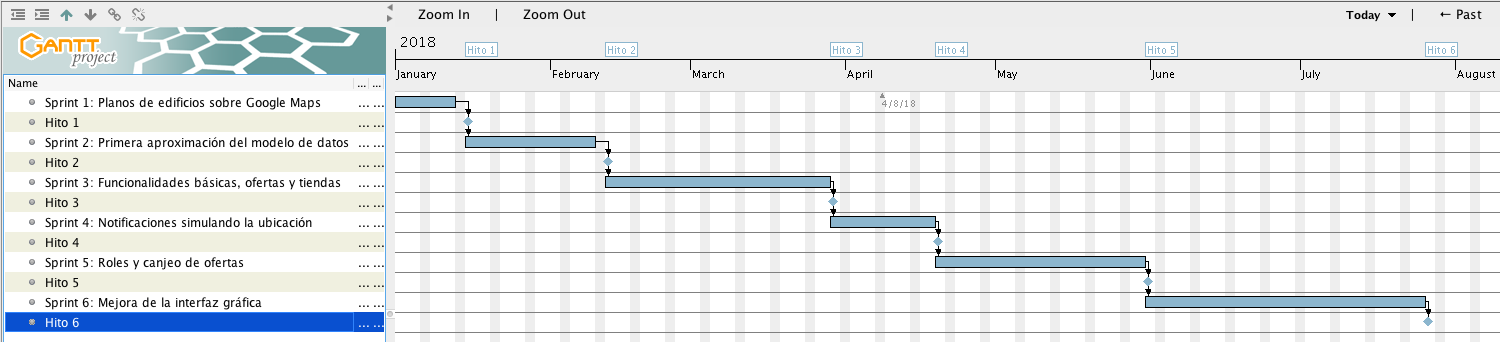
\includegraphics[width=\textwidth]{figures/gantt-final.png}
\caption{Diagrama de \textit{Gantt} final del proyecto.
\label{fig:gantt_final}}
\end{center}
\end{figure}

\section{Evaluación de costes}
A partir de la planificación inicial y de los recursos materiales y humanos necesarios, podemos hacer una estimación de lo que valdría el proyecto en un entorno empresarial.

\subsection{Costes materiales y \textit{software}}
En este proyecto hemos utilizado materiales de los que ya disponíamos y que además ya se encontraban amortizados en el momento de su utilización.
El \textit{software} utilizado también fue gratuito, o bien de pago en su versión de prueba.
Pero hay que mencionar a parte los servicios de \textit{Firebase Database}, \textit{Google Maps} y \textit{Situm}. Ya que en caso de que la aplicación quisiese lanzarse al público, habría que contratar unas tarifas que dieran soporte a mayor número de usuarios, a continuación unas tablas que muestra sus precios:
\begin{table}[btp]
\begin{center}
\small
\begin{tabular}{|l|l|l|l|}
\hline 
& Plan Spark & Plan Flame & Plan Blaze \\
\hline \hline
Precio & Sin cargo & USD 25/mes & Pago por uso \\ \hline
Conexiones simultáneas & 100 & 100.000 & 100.000 por  base de datos \\ \hline
GB almacenados & 1 GB & 2,5 GB & USD 5/GB   \\ \hline
GB descargados & 10 GB/mes & 20 GB/mes & USD 1/GB   \\ \hline
Varias bases de datos  & No & No & Sí  \\ \hline
\end{tabular}
\caption{Precios de \textit{Firebase Database}.}
\label{precios:firebase_db}
\end{center}
\end{table}

\begin{table}[btp]
\begin{center}
\small
\begin{tabular}{|l|l|c|}
\hline 
& Uso mensual gratis & Precio  \\
& (por valor de USD 200) &  por cada mil llamadas \\
\hline \hline
Mapas estáticos & 100.000 cargas & USD ~2 \\ \hline
Mapas dinámicos & ~28.000 cargas & USD ~7 \\ \hline
Street View Estático & ~28.000 panorámicas & USD ~7   \\ \hline
Street View Dinámico & ~14.000 panorámicas & USD 14   \\ \hline
\end{tabular}
\caption{Precios de \textit{Google Maps} de 0 a 100.000 llamadas mensuales.}
\label{precios:googlemaps}
\end{center}
\end{table}

Cuando el intervalo de llamadas mensuales está entre 100.000 y 500.000 a la \textit{API} de \textit{Google Maps}, los precios por cada mil llamadas disminuyen un 20 por ciento con respecto al intervalo 0 - 100.000. Y cuando las llamadas mensuales superan los 500.000, entonces debemos ponernos en contacto con ventas para estipular el precio.

\begin{table}[t]
\begin{center}
\small
\begin{tabular}{|l|c|c|}
\hline 
& Estándar & Premium \\
\hline \hline
Precio & Gratis & 29,90 euros/mes \\ \hline
Posicionamiento preciso 3D & Sí & Sí \\ \hline
Navegación interior paso a paso & Sí & Sí \\ \hline
Creación/subida de ilimitados edificios/mapas & Sí & Sí   \\ \hline
Creación de Puntos de Interés, interiores y exteriores & Sí & Sí  \\ \hline
Creación de Rutas convencionales y accesibles & Sí & Sí   \\ \hline
Generación de eventos/Diseño estrategia geomarketing & Sí & Sí   \\ \hline
Análisis de informes y estadísticas de uso & Sí & Sí  \\ \hline
Visualización de usuarios en tiempo real & Sí & Sí  \\ \hline
Disponible sólo para evaluación & Sí & Sí   \\ \hline
Uso comercial & No & Sí   \\ \hline
Soporte premium & No & Sí   \\ \hline
Alta disponibilidad & No & Sí   \\ \hline
Servicio para empresas & No & Sí   \\ \hline
\end{tabular}
\caption{Precios de \textit{Situm}.}
\label{precios:situm}
\end{center}
\end{table}

\paragraph{Tarifas \textit{Postman}}
Se ha utilizado la versión gratuita de este programa y fue más que suficiente. Pero también tiene opciones de pago  (figura~\ref{fig:postman_pricing}).

\paragraph{Tarifas \textit{Adobe Xd}}
La herramienta de diseño \textit{Adobe Xd} puede utilizarse de manera gratuita, pero también hay opciones de pago que ofrecen funcionalidades más amplias (tabla~\ref{fig:adobe_pricing}).

\begin{table}[t]
\begin{center}
\small
\begin{tabular}{|l|c|c|c|c|}
\hline 
Plan & Precio & Llamadas incluidas & Llamadas & Llamadas\\
& (usuario/mes) & por mes & a mayores & bajo demanda\\ \hline \hline
Postman & 0 USD & 1000 al mes & - & - \\ \hline
Postman & 8 & 10000 & 20 USD/mes & 0.75 USD\\
Pro & USD & al mes & por 50000 &  por 1000\\ \hline
Postman & 18 & 100000 & 20 USD/mes & 0.75 USD\\ 
Enterprise & USD & al mes & por 50000 & por 1000 \\ \hline
\end{tabular}
\caption{Tarifas y planes de uso de la herramienta \textit{Postman}.}
\label{fig:postman_pricing}
\end{center}
\end{table}

\begin{figure}[t]
\centering
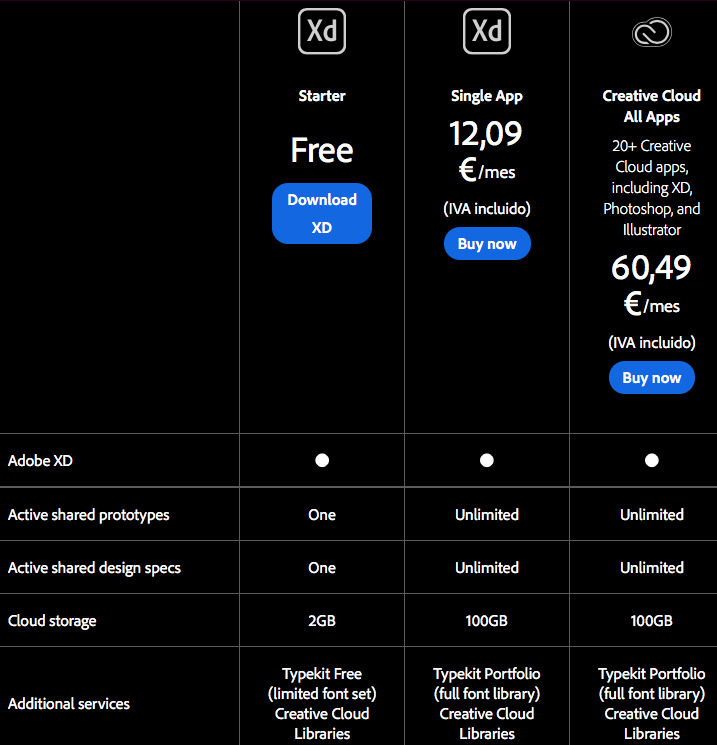
\includegraphics[scale=0.45]{figures/adobe-pricing.png}
\caption{Tarifas de la herramienta de diseño \textit{Adobe Xd}.
\label{fig:adobe_pricing}}
\end{figure}

\subsection{Costes de recursos humanos}
Al ser el equipo de desarrollo de un sólo integrante, no era necesario cumplir con un horario regular, así que para estimar las horas empleadas en el proyecto vamos a asumir que se le dedicaron unas 80 horas mensuales desde Marzo hasta Agosto, ambos inclusive. Además se realizaron 10 reuniones con el director de proyecto, cada una de las cuales, de una duración aproximada de 2 horas. Este último, también cumplía las funciones de consultor y analista así que habrá que tenerlas en cuenta.
\begin{table}[bt]
\begin{center}
\small
\begin{tabular}{|l|c|c|c|}
\hline 
Recurso & Salario (euros/hora) & Horas empleadas & Coste (euros) \\
\hline \hline
Jefe de proyecto & 60 & 20 & 1.200 \\ \hline
Analista & 40 & 90 & 2.000 \\ \hline
Programador & 30 & 400 & 15.200 \\ \hline
\end{tabular}
\caption{Precios estimados de los recursos humanos empleados en el proyecto.}
\label{precios:rrhh}
\end{center}
\end{table}






